%%%%%%%%%%%%%%%%%%%%%%%%%%%%%%%%%%%%%%%%%%%%%%%%%%%%%%%%%%%%%%%%%
%_____________ ___    _____  __      __ 
%\____    /   |   \  /  _  \/  \    /  \  Institute of Applied
%  /     /    ~    \/  /_\  \   \/\/   /  Psychology
% /     /\    Y    /    |    \        /   Zuercher Hochschule 
%/_______ \___|_  /\____|__  /\__/\  /    fuer Angewandte Wissen.
%        \/     \/         \/      \/                           
%%%%%%%%%%%%%%%%%%%%%%%%%%%%%%%%%%%%%%%%%%%%%%%%%%%%%%%%%%%%%%%%%
%
% Project     : Bachelorarbeit
% Title       : Einleitung
% File        : einleitung Rev. 00
% Date        : 06.12.2013
% Author      : Till J. Ernst
%
%%%%%%%%%%%%%%%%%%%%%%%%%%%%%%%%%%%%%%%%%%%%%%%%%%%%%%%%%%%%%%%%%
\glsresetall % zurücksetzen der Acronyms
\let\raggedsection\centering
\chapter{Einleitung (Gegenwart)}\label{chap.einleitung}
\let\raggedsection\raggedright 
%####################################################
% Kapitel Ausgangslage
%####################################################
\section{Ausgangslage}\label{section.einleitung.ausgangslage}
In den letzten Jahren ist der Medienkonsum unter Jugendlichen und Erwachsenen rasant angestiegen \cite{Shih2013}. Ein Grund dafür ist die leichte Zugänglichkeit von Medien über neue Technologien wie Smartphones, Tablets und Computer. In einer gross angelegten Studie der Kaiser Family Foundation \cite{Rideout2010}, in der über 2000 8- bis 18-Jährige zu ihrem Medienverhalten befragt wurden, konnte festgestellt werden, dass die Gesamtzeit, in der die Jugendlichen Medien ausgesetzt sind, im Jahr 2009 auf 10 Stunden und 45 Minuten pro Tag angestiegen ist. Im Jahr 1999 waren es noch 7 Stunden und 29 Minuten. Dies entspricht einem Anstieg von 44\% innerhalb von einem Jahrzehnt. Die eigentliche Mediennutzung dieser Jugendlichen stieg von 6 Stunden und 19 Minuten im Jahr 1999 auf 7 Stunden und 38 Minuten im Jahr 2009 an. Diese entspricht beinahe der Arbeitszeit, die Erwachsenen pro Tag auf der Arbeit verbringen \cite{Rideout2010}. In der Schweiz gehören digitale Medien zu den beliebtesten Freizeitaktivitäten der Jugendlichen. Dazu gehören Medien wie das Mobiltelefon, Internet und Musik hören. Wobei das Mobiltelefon das am meisten genutzte Medium darstellt \cite{Willemse2012}. Die universelle Medienbenützung wird zu einem globalen Phänomen. Nicht nur jugendliche sind von diesem Trend betroffen, vielmehr handelt es sich hierbei um eine Entwicklung, die in allen Altersgruppen und Berufsgruppen anzutreffen ist \cite{Rogers2009}. Diese Mediennutzung hat längst Einzug in unseren Arbeitsstätten und Klassenräumen gehalten und hat uns ein Stückweit den Weg gewiesen, wie wir untereinander Kommunizieren und interagieren \cite{Benson2002}. Dieser Anstieg der Mediennutzung lässt die Frage nach möglichen Auswirkungen des Medien-Konsums auf die psychische Gesundheit und kognitive Funktion entstehen. Aktuelle Forschungsergebnisse lassen jedoch noch keinen eindeutigen Schluss auf diese Frage zu. Einführende Studien deuten darauf hin, dass sich die Befürchtung einer Verschlechterung der Psyche und der Hirnfunktionen bewahrheitet \cite{Biocca2000, Roberts2008}. Im Forschungsbereich der psychischen Gesundheit wurden Anzeichen für einen Zusammenhang zwischen Medienkonsum und negativ einhergehendem sozialem Wohlbefinden und verminderten psychosozialen Funktionen gefunden \cite{Kraut1998, Moody2001}. Im Bildungsbereich wurden Anzeichen für einen möglichen Medien-Einfluss auf das Lernverhalten festgestellt \cite{Prensky2001}. In den meisten bisherig erwähnten Forschungsergebnissen wurde das Ausmass anhand der eigentlichen Medien-Nutzungsdauer untersucht. Dabei spielt das simultane Benützen mehrerer Medien eine immer grösser werdende Rolle \cite{Jeong2007}. Währendem die absolute Nutzungsdauer in den vergangenen Jahren rapide angestiegen ist, so konnte bei dieser Art von Mediennutzung erst recht eine Steigerung festgestellt werden. Im letzten Jahrzehnt hat sich das Verhältnis von Medien-Multitasking (das gleichzeitige Benutzen mehrere Medien) gegenüber der eigentlichen Mediennutzung von 16\% in 1999 auf 29\% in 2009 gesteigert \cite{Rideout2010}. Dieser rasante Anstieg wirft erneut die Fragen betreffend den möglichen Auswirkungen auf die Gedächtnisleistung und die psychische Gesundheit auf \cite{Alzahabi2013}. 

%####################################################
% Kapitel Hintergrund, Begründung und Ziel der Studie
%####################################################
\section{Hintergrund, Begründung und Ziel der Studie}\label{section.einleitung.hintergrund}
Zahlreiche Studien haben sich bereits mit den Auswirkungen von Medien-Nutzung auf die kognitive und psychische Entwicklung befasst und konnten wichtige Erkenntnisse dazu liefern \cite<z.B.: >{Prensky2001, Biocca2000, Roberts2008}. Im Schnittpunkt von Wohlbefinden und dem Medien-Nutzverhalten im aktuellen Bereich des Medien-Multitasking wurde bisher wenig Forschung betrieben \cite{Pea2012}. Ausgehend von den wenig bereits existierenden Studien über die Auswirkungen von \gls{labelMMT} geht hervor, dass \gls{labelMMT} einmalig im Bezug zu den Auswirkungen auf die psychische Gesundheit und die kognitiven Funktionen sei \cite{Joeng2007}. Aktuelle Studien legen nahe, dass \gls{labelMMT} mit höheren Symptomen von Depression und sozialer Angst \cite{Becker2013} und ansteigendem Medien-Konsum einhergeht. Ebenso soll das soziale Wohlbefinden von Mädchen mit steigendem \gls{labelMMT} abnehmen \cite{Pea2012}. Bezüglich kognitiven Prozessen konnten negative Auswirkungen von Multitasking auf die Schulleistung gefunden werden \cite{Junco2012}. In einem Laborversuch von \citeA{Ophir2009} konnte ein Zusammenhang mit Medien-Multitasking und kognitiver Leistung nachgewiesen werden. Diese Studie legt nahe, dass starke Medien-Multitasker Mühe haben, zwischen einzelnen Aufgaben hin und her zu wechseln. Diese Multitasker mussten mehr Leistung für diesen Wechsel aufwenden, als moderate oder schwache Medien-Multitasker. Eine mögliche Erklärung für dieses Ergebnis könnte sein, dass das häufige Praktizieren von Medien-Multitasking die Fähigkeit der Nutzer für das simultane Verarbeiten von Informationen steigert, indes die Notwendigkeit vom Wechsel zwischen Aufgaben verringert und somit die Übung für diesen Wechsel bei starken Multitasker ausbleibt \cite{Alzahabi2013, Watson2010}. Aus den erwähnten Studien geht hervor, dass der kognitiven Komponente einige Forschungsarbeiten gewidtmet wurde. Die Auswirkungen von Medien-Multitasking auf das subjektive Wohlbefinden hingegen, ist in der aktuellen Forschung wenig vertreten. Eine aktuelle Studie um \citeA{Shih2013} mit 138 Studenten konnte keinen relevanten Zusammenhang zwischen Medien-Multitasking und dem Wohlbefinden herstellen. Trotz diesem Ergebnis ist klar, dass hier weitere Studien folgen müssen. Das Ziel dieser Bachelorarbeit ist es, einen Teil dieser Forschungslücke zu schliessen. Es soll die Auswirkung von Medien-Multitasking auf das subjektive Wohlbefinden näher untersucht und beleuchtet werden. 

%####################################################
% Kapitel Aufbau der Arbeit
%####################################################
\section{Aufbau der Arbeit}\label{section.einleitung.aufbau}
Diese Arbeit beginnt mit einem einleitenden Kapitel, in dem theoretische Konstrukte und der aktuelle Forschungstand erläutert werden. Darin werden die Begriffe Multitasking und subjektives Wohlbefinden mit den für diese Arbeit weiteren relevanten Konstrukten erklärt. Aktuelle Forschungsergebnisse sollen weiter in die Thematik verhelfen und mögliche Forschungslücken aufzeigen. Abschliessend wird die Forschungsfrage und die daraus resultierende Hypothese hergeleitet. Im Methodenteil folgen Angaben über das eigentliche Studiendesign, die Auswahl der Stichprobe und die verwendeten Messmittel, um den daraus resultierenden Online-Fragebogen zu erstellen. Weiter wird die eigentliche Datenerhebung, die Datenaufbereitung und die dazu notwendigen statistischen Verfahren erläutert. Die Ergebnisse werden anhand der gefundenen Daten dargestellt und gemäss einleitender Hypothesen wiedergegeben und Analysiert. Im Abschliessenden Teil dieser Arbeit werden die Ergebnisse in Bezug zu den Fragestellungen gesetzt und interpretiert. Es folgt eine Methodenkritik und einen Ausblick für weiterführende Untersuchungen.

%####################################################
% Kapitel Theoretischer Hintergrund
%####################################################
\section{Theoretischer Hintergrund}\label{section.einleitung.theoHintegrund}
Der theoretische Hintergrund dient zur Erläuterung von Begriffen, Konstrukten und Definitionen, auf denen diese Arbeit aufgebaut ist. In einem ersten Teil werden Begriffsbestimmungen und Definitionen behandelt. Anschliessend werden die beiden Konstrukte Medien-Multitasking und subjektives Wohlbefinden ausführlich erläutert. Diese Konstrukte bilden aus theoretischer Sicht die beiden Schwerpunkte dieser Arbeit.
% Begriffsbestimmungen, Definitionen ---------------------
\subsection{Begriffsbestimmungen, Definitionen}
\label{subsection.begriffsbestimmung}
\textbf{Sensation Seeking:}
Die Suche nach starken Reizen, wie dieses Konzept von \citeA{Zuckerman2006} auch umschrieben wird. Es geht hierbei um die Suche nach Abwechslung und neuen Erlebnissen. Streben nach starken Reizen und stimulierenden Erfahrungen, um Spannungsreize zu erleben. Diese Verhaltensdisposition basiert auf genetischer und biochemischer Basis. Dieses Konstrukt geht auf Freuds Konzept der Trieb oder Spannungsreduktion sowie auf das Modell der optimalen Stimulation und Erregung zurück \cite{Doernhaus2014}. 
\par
\textbf{Digital Natives und Digital Immigrants:} Im Umgang mit Medien und der daraus resultierenden Medienkompetenz wird oft anhand der Generationsgestaltung eine Unterteilung nach Alterskohorten vorgenommen \cite{Suss2013}. In dieser Unterteilung geht es darum, unterschiedliche Bedingungen während dem Erwachsenwerden in bestimmten Alterskohorten anhand wirtschaftlicher, kultureller, sozialer und politischen Entwicklungen, gegenüber einer früher geborenen Kohorte zu unterscheiden. Gemäss \citeA{Suss2004} werden diese Unterteilungskriterien mit den Leitmedien der jeweiligen Zeiträume in Verbindung gesetzt. Leitmedien sind Medien, die eine hohe Verbreitung haben, intensiv genutzt werden, zahlreiche Funktionen bereitstellen und zu denen eine hohe Bindung aufgebaut werden kann \cite{Suss2013}. \textit{Digital Natives} sind Menschen, die mit den neunen Informations- und Kommunikationstechnologien aufgewachsen sind. \textit{Digital Immigrants} sind hingegen Menschen, welche diese digitalen Medien erst im Erwachsenenleben kennen gelernt haben \cite{Prensky2001}. Die Unterteilung dieser beiden Kohorten wird gemäss \citeA{Suss2013} anhand der \textit{Net Generation} vorgenommen, die um 1985 geboren ist. Diese Generation wird als Digital Natives bezeichnet, die diese besondere Affinität zu Computer- und Videospielen als Freizeitbeschäftigung aufweist.
\par
\textbf{Polychronizität:}
Bei Polychronizität handelt es sich um ein mit dem Multitasking verwandtes Konzept. Es beschreibt die Vorliebe, mehrere Aufgaben zur selben Zeit zu erledigen und zu bearbeiten \cite{Baethge2010}. Polychronizität bezieht sich auf die Neigung, die eigene Zeit einzuplanen und zu strukturieren \cite{Hecht2005}. Einige bevorzugen es, sich auf eine Aufgabe auf einmal zu konzentrieren, andere hingegen bevorzugen es, sich auf mehrere Aufgaben gleichzeitig zu konzentrieren. Das Konzept wurde 1959 erstmals von \cite{Hall1980} beschrieben. In den frühen Arbeiten zur Polychronizität wurde diese als kulturelles Phänomen behandelt. Hall definierte zwei Gruppen, die er anhand der Vorliebe für deren Zeiteinteilung benannte: Monochronisch und polychronisch. Seit den 1990er Jahren steht nicht mehr die Kultur im Mittelpunkt, vielmehr steht das Individuum im Fokus \cite{Baethge2010}.

% Medien-Multitasking ---------------------
\subsection{Medien-Multitasking}\label{subsection.medienMultitasking}
Unter \gls{labelMMT} wird das Erledigen von mehr als einer Medienaktivität zur selben Zeit verstanden, wie zum Beispiel das Schreiben von Email, das Versenden von Instant-Nachrichten, das Lesen von Online-Zetischriften oder andere computer basierte Tätigkeiten \cite{Foehr2006}. Medien-Multitasking ist eine spezifische Form von \gls{labelMT}, was im Grunde genommen das Erledigen vieler (aus dem Lateinischen von \textit{multi}) Aufgaben (aus dem Englischen von \textit{task}) zur gleichen Zeit bedeutet \cite{Spitzer2012}.  Im Folgenden wird aus theoretischer Sicht auf dieses Verhalten eingegangen. In einem ersten Teil wird eine Übersicht verschiedener Theorien gegeben. Anschliessend werden einzelne Konstrukte wie die Aufmerksamkeit und das Arbeitsgedächtnis näher beleuchtet. Abschliessend wird auf das Medien-Multitasking im spezifischen eingegangen.
\par
\textbf{Multitasking, eine kurze theoretische Übersicht:} Ursprünglich stammt das Wort Multitasking aus dem Computer-Bereich und beschreibt die Fähigkeit eines Betriebssystems, mehrere Aufgaben praktisch gleichzeitig auszuführen \cite{Multitasking2010}. Es scheint, als ob neue Technologien wie Computer und mobile Endgeräte das obsessive Wechseln zwischen verschiedenen Aufgaben fördern würden. Eine Untersuchung an Arbeitsplätzen in den USA hat ergeben, dass die Angestellten ungefähr jede dritte Minute einer Unterbrechung oder Ablenkung ausgesetzt sind und dass Personen, welche an einem Computer arbeiten, durchschnittlich acht verschiedene Programmfenster geöffnet haben \cite{Thompson2005}. Daraus geht hervor, dass ständige Ablenkung, die in Form von Eindrücken und Informationen (Reizen) auf diese Personen eingeht, eine gewachsene Anforderung in der heutigen Zeit darstellt \cite{Klingberg2008}. Innerhalb der Psychologie und der Hirnforschung wurde festgestellt, dass die Probleme beim Multitasking auf eine einzige zentrale Beschränkung zurückzuführen ist: Die Fähigkeit, Informationen unmittelbar im Gedächtnis zu behalten \citeyear<ebda.,>{Klingberg2008}. Es gibt wenig Übereinstimmung in der neurologischen und psychologischen Literatur, wenn es darum geht, die Verarbeitung von mehr als eine Nachricht oder die Ausführung mehrerer Aufgaben gleichzeitig, anhand von Funktionsprinzipien im Gehirn zu definieren und zu beschreiben \cite{Kieras1997}. Viele Informationsverarbeitungstheorien basieren auf einer Limitierung der gleichzeitigen Informationsverarbeitung im Gehirn \cite{Kieras1997, Pashler2000}. Untersuchungen haben gezeigt, dass zwar zwei gleichzeitige Stimuli im Gehirn eingehen können, diese aber nicht simultan bearbeitet werden können \cite{Pashler2000}. Diese Phänomen wird als \gls{labelPRP} bezeichnet \cite{Welford1952} und bezeichnet den Zeitintervall, der zusätzlich vergeht, um einen Reiz zu verarbeiten, der unmittelbar nach einem vorhergehenden Reiz eingetroffen ist. Es wurden jedoch auch Reize gefunden, bei denen keine solche Verzögerung auftritt \cite{Foehr2006}. Forscher sind sich uneins, was genau die Minimierung der parallelen Informationsverarbeitung verursacht. Viele schreiben diese Kapazitätsgrenze dem Auffinden von Informationen im Gehirn zu oder der Planung der nächsten Handlungen, ohne jedoch genau zu wissen, wie simultane Aufgaben wirklich verarbeitet werden \cite{Kieras1997}. Einige Forscher spekulieren auf eine zentrale Verarbeitungs-Einheit, die Aufgaben in einer Liste verwaltet. Andere gehen davon aus, dass es sich um den limitierenden Faktor handelt, das nicht mehr als eine aktive Zuordnung einer Aufgabe im Gehirn bewerkstelligt werden kann \cite{Pashler2000}. Eine der Hauptbelastungen im Zusammenhang mit Multitasking hat mit Gehirn-Ressourcen zu tun. Mittels Magnetresonanztomographie konnte bei Probanden nachgewiesen werden, dass das Aktivitätsvolumen bei zwei simultan ausgeführten Aufgaben im Gehirn signifikant kleiner ist, als wenn diese beiden Aktivitäten unabhängig voneinander ausgeführt und die beiden Aktivitätsvolumen im Nachhinein addiert wurden \cite{Just2001, Klingberg1997}. Dieser Befund spricht für die Verarbeitung von verschiedenen Aufgaben im selben Bereich des Gehirns \cite{Klingberg1997}, sowohl für die Trennung nach räumlichen Beziehungen sowie der semantischen Kategorisierung \cite{Just2001}. Eine Interpretation dieses Befundes lässt den Schluss zu, dass im Gehirn eine Höchstgrenze an aktivem Hirngewebe für das Lösen von Aufgaben zu einem Zeitpunkt vorhanden ist. Wenn also zwei Aufgaben simultan verarbeitet werden, werden reduzierte Ressourcen für je eine Aufgabe aufgewendet \cite{Just2001}. Eine weitere Interpretation dieser Resultate schlägt eine Limitierung der Aufmerksamkeit vor, die eine Person erbringen kann \citeyear<ebda.,>{Just2001}. Somit ist der Limitierende Faktor für das simultane Bearbeiten von Aufgaben die Aufmerksamkeitskontrolle. Dieser Erklärungsmodell deckt sich auch mit derjenigen von \citeA{Lang2000} und anderen Theorien der Informationsverarbeitung \cite{Kieras1997}. Weitere Studien haben ergeben \cite{Grimes1990} dass semantisch identische Informationen (wie zum Beispiel Audio- und Visuelle-Informationen in einer Informationssendung) von Benutzern gut gefolgt und deren Information mit Leichtigkeit wiedergegeben werden können (perzeptueller Gruppierungsvorgang). Wohingegen bei semantisch unterschiedliche Kanälen, die Benutzer mehr Mühe haben sich auf einen Kanal zu konzentrieren und im Nachhinein Informationen abzurufen.
\par
\textbf{Verschiedene Arten von Aufmerksamkeit:} Aus der vorhergehenden Theorieübersicht geht hervor, das Multitasking etwas mit Konzentration zu tun hat, indem die Aufmerksamkeit bewusst oder unbewusst auf spezifische Aufgaben oder Informationen gelenkt wird (die beiden Begriffe Aufmerksamkeit und Konzentrationsfähigkeit werden in dieser Arbeit synonym verwendet) \cite{Klingberg2008}. Es werden mindesten drei Arten von Aufmerksamkeit unterschieden: Dies ist die \textit{kontrollierte Aufmerksamkeit}, die eingesetzt wird wenn eine willentliche Aufgabe gelöst wird. Der zweite Aufmerksamkeitstyp ist die \textit{reizbedingte Aufmerksamkeit}, welche automatisch auf eintretende Reize in der Umgebung gelenkt wird und als dritter Typ gilt der allgemeine \textit{Wachheitsgrad}, der die Aufmerksamkeit mit fortschreitender Müdigkeit stärker beeinflusst \cite{Posner1978}. Für die kontrollierte und für die reizbedingte Aufmerksamkeit konnten zwei parallele System im Gehirn ausfindig gemacht werden, die voneinander unabhängig sind \cite{Corbetta2002}. Durch Untersuchungen mit Personen, die in dem Bereich der Scheitellappen Läsionen aufwiesen,  konnte festgestellt werden, dass Einschränkungen in der Fähigkeit des Gehirns Informationen aufzunehmen, mit den Mechanismen der Aufmerksamkeit erklärt werden konnten \cite{Klingberg2008}.
\par
\textbf{Das Arbeitsgedächtnis:} Im Zusammenhang mit der kontrollierten Aufmerksamkeit steht das Arbeitsgedächtnis, welches durch gezielte Anweisung die Aufmerksamkeit dazu veranlasst, sich auf eine Sache zu konzentrieren. Das Arbeitsgedächtnis besitzt die Fähigkeit, Informationen für einen kurzen Zeitraum im Kopf zu behalten \cite{Klingberg2008}. Gemäss \citeA{Baddeley2003} beinhaltet das Arbeitsgedächtnis drei gesonderte Subsysteme: Eines ist zuständig für die Speicherung visueller Informationen, ein zweiter Bereich ist zuständig für die Verarbeitung von verbaler Informationen und ein dritter Bereich, die zentrale Executive, koordiniert die Funktionen der beiden anderen. Arbeitsgedächtnisaufgaben werden unterschieden zwischen eher passiven Aufgaben, die eine Form von Ablenkung enthalten, beziehungsweise ein gewisses Mass an Multitasking erfordern, und eher aktiven Aufgaben, die eine gewisse Art der Manipulation erfordern \cite{Klingberg2008}. Das Mass an Informationen, die gleichzeitig verarbeitet werden können, hängt demzufolge vom Arbeitsgedächtnis ab. Die Kapazität des Arbeitsgedächtnis nimmt während der gesamten Kindheit zu und erreicht ihren Höhepunkt im Alter von etwa 25 Jahren. Danach nimmt das Arbeitsgedächtnis kontinuierlich ab\cite{Swanson1999}.
\par  
\textbf{Multitasking und mentale Bandbreite:} Das scheinbar gleichzeitige Erledigen zweier Aufgaben ist dadurch erschwert, dass Informationen immer nur von einer Stelle zur gleichen Zeit aufgenommen werden können. Gewisse Aufgaben lassen sich nur sehr schwer gleichzeitig durchführen, weil gleichartige Verarbeitungsprozesse  benötigt werden (Stimulus und Response)\cite{Klingberg2008}. Durch Tests konnte nachgewiesen werden, dass die Einschränkung beim Multitasking mit dem Arbeitsgedächtnis zusammenhängt und dass die Ablenkbarkeit steigt, je stärker eine Aufgabe oder Handlung das Arbeitsgedächtnis beansprucht \cite{Lavie2005}. Somit kann gesagt werden, dass je stärker das Arbeitsgedächtnis ausgelastet ist, desto leichter fühlt man sich abgelenkt und gestört. Ein hoher Grad an Ablenkung stellt somit eine höhere Anforderung an das Arbeitsgedächtnis, dessen Belastungsgrad demzufolge für die erfolgreiche Verarbeitung von Multitasking Aufgaben verantwortlich ist \cite{Klingberg2008}.
\par
\textbf{Multitasking und Gender:}
Können Frauen besser Multitasking betreiben als Männer? Diese etwas salopp formulierte Frage wird oftmals diskutiert, mit teilweise unterschiedlichen Ergebnissen. Die allgemeine Meinung schreibt den Frauen eine höhere Multitasking-Fähigkeit zu als den Männern \cite{Oconnell2002}. Eine Erklärung zur Unterstützung dieser These ist, dass Frauen einen grösseren präfrontalen Kortex haben, der für das Multitasking verantwortlich ist, und somit von der Bauform des Gehirns besser für das Multitasking ausgelegt sind \cite{Fisher2000}. Eine weitere Erklärung im Bereich der Evolutionspsychologie lautet, dass Frauen für den Nachwuchs sorgen mussten, somit mit einer Vielzahl unterschiedlicher Aufgaben konfrontiert wurden und nur diejenigen überlebten, die diese Aufgabe erfolgreich ausführen konnten \cite{Ellison2006}. Trotz diesen Erklärungen existiert wenig an Forschung in diesem Bereich. \citeA{Schneider2005, Foehr2006} konnten in ihren Studien nachweisen, dass Frauen tendenziell mehr Multitasking betreiben als Männer. Wissenschaftlich kann die Frage bis jetzt noch nicht schlüssig beantwortet werden \cite{Foehr2006}. Es ist nach wie vor nicht bekannt, wer nun wirklich besser Multitasking betreiben kann \cite{Mahany2005, Klingberg2008}. 
\par  
\textbf{Gehirnareale und kognitive Strukturen:} Multitasking beanspruchen vor allem das Arbeitsgedächtnis und die Aufmerksamkeit \cite{Baethge2013}. Personen mit höherer Arbeitsgedächtnis-, Aufmerksamkeitsleistung schneiden auch in Aufgaben mit Multitasking besser ab \cite{Buhner2006}. Zusammenfassend können folgende Gehirnareale und kognitive Strukturen für die Beteiligung an Multitasking benannt werden: Beteiligte neurologische Strukturen sind vor allem der Präfrontale Kortex mit den Arealen Anteriorer Cingulärer Kortex und Dorsolateraler Präfrontalkortex \cite{Dreher2003}.
\par
\textbf{Medien-Multitasking:} Der Name Medien-Multitasking umfasst eine Vielzahl von unterschiedlichen Medien-Aufgaben, die gleichzeitig verarbeitet werden. In vielen solcher gleichzeitigen Aufgaben geht es nicht unbedingt darum, nicht zusammenhängende Informationen simultan zu verarbeiten und zu gruppieren (perzeptueller Gruppierungsvorgang). Vielmehr wird zwischen den einzelnen, unterschiedlichen Aufgaben hin und her gewechselt. Neurologen konnten dieses Gebiet im präfrontalen Cortex des Gehirns festlegen, welches für diesen Wechsel zwischen den Aufgaben zuständig ist \cite{Wallis2006, Wood2003}. Über die Auswirkung von diesem hin und her Wechseln zwischen Aufgaben ist bis dato noch nicht viel bekannt. Der Fokus lag und liegt oftmals in der Identifizierung von negativen Effekten von Medien-Multitasking. Es wäre aber auch durchaus möglich, dass die Auseinandersetzung mit unterschiedlichen Medien gleichzeitig einen positiven Effekt haben könnte \cite{Foehr2006}.   

% Subjektives Wohlbefinden ---------------------
\subsection{Subjektives Wohlbefinden}\label{subsection.subjektivesWohlbefinden}
In diesem Abschnitt wird auf das \gls{labelSWB} und die damit Verbundenen Konzepte eingegangen. Subjektives Wohlbefinden und Wohlbefinden wird in der Literatur sehr unterschiedlich verwendet. Wenn in dieser Arbeit die Rede von Glück im Sinne von \gls{labelSWB} ist, so wird immer die Bedeutung im Sinne der Erfüllung gemeint. Glück im Sinne des Zufalls ist nicht psychologisch und somit für diese Arbeit nicht relevant. \Gls{labelSWB} wird in dieser Arbeit als ein Konstrukt der positiven Psychologie verstanden. 
\par
\textbf{Positive Psychologie:} 
Klinische Psychologie legt den Fokus traditionsbedingt vorwiegend auf menschliche Defizite und psychische Behinderungen. Die Resilienz von Patienten, Ressourcenorientierung und die Fähigkeit zur Regeneration wurden lange Zeit vernachlässigt \cite{Carr2011}. Mit der Einführung der positiven Psychologie, bei der allgemein der amerikanische Professor Martin E.P. Seligman und seine Kollegen als Begründer gilt \cite{Seligman2003}, wurde die defizit-orientierte Psychologie ergänzt. Dieser neue Zweig der Psychologie befasst sich primär mit den menschlichen Stärken und dem menschlichen Glück aus wissenschaftlicher und klinischer Sicht \cite{Carr2011}. Die wissenschaftliche Auseinandersetzung innerhalb der Positiven Psychologie befasst sich mit dem Verstehen und dem Verbessern von positiven Aspekten im Leben:
\begin{itemize}
    \item Glück und Wohlbefinden,
    \item positive menschliche Eigenschaften und Engagement in absorbierenden Aktivitäten, und
    \item der Entwicklung von positiven Beziehungen, sozialen Systemen und sozialen Einrichtungen \cite{Lopez2009, Seligman2003}.
\end{itemize}
Die positive Psychologie widmet sich der Erforschung des \textit{angenehmen Lebens} (engl. pleasant life), des \textit{engagierten Lebens} (engl. engaged life) und des \textit{bedeutungsvollen Lebens} (engl. meaningful life). Diese drei Faktoren führen zum Glück und sind für das Wohlbefinden eines Menschen zuständig \cite{Peterson2005}. Das klinische Bestreben der Positiven Psychologie hat weniger das Korrigieren von Defiziten zum Ziel, sondern die Steigerung von Wohlbefinden und Glück. Vielmehr soll sie zur Vervollständigung und nicht zum vollständigen Ersatz der Klinischen Psychologie beitragen \cite{Carr2011}.
\par
\textbf{Positive Emotionen und Glück:} 
Gemäss \citeA{Seligman2003} werden die Worte \textit{Glück} oder \textit{Glücklichsein} und \textit{Wohlbefinden} als synonym und austauschbar angesehen. Sie sind übergreifende Begriffe, die die Ziele der gesamten positiven Psychologie beschreiben. Sie umfassen beides: Positive Gefühle, wie Ekstase oder Behagen, sowie positive Verhaltensweisen, die keine Gefühlskomponenten besitzen, wie Absorption oder Engagement. Die gewünschten Ergebnisse der positiven Psychologie sind Glück und Wohlbefinden.\\
\citeA{Seligman2003} teilt die Emotionen, die zur Steigerung des Glücks beitragen, in drei Gruppen ein: Die einen beziehen sich auf die Vergangenheit, die anderen auf die Zukunft, die dritten auf die Gegenwart. Vergangenheitsbezogene Emotionen sind unter anderem Genugtuung, Zufriedenheit, Stolz und Gelassenheit. Optimismus, Hoffnung, Vertrauen, Glauben und Zuversicht sind Emotionen, die den zukunftsorientierten Emotionen zugeordnet werden können. Bei den gegenwartsbezogenen Emotionen lassen sich weiter zwei grundlegend verschiedene Unterkategorien bilden: Momentane \textit{Vergnügen} oder \textit{Genüsse} und die eher überdauernden \textit{Belohnungen}. Vergnügen und Genüsse umfassen körperliche und höhere Vergnügen. Körperliche Vergnügen sind momentane positive Emotionen, die über die Sinneswahrnehmungen vermittelt werden, wie delikate Geschmacksempfindungen und Gerüche, sexuelle Gefühle, elegante Körperbeherrschung, reizende Anblicke und Geräusche oder Töne. Die höheren Vergnügen sind ebenfalls zeitlich begrenzt, werden aber durch komplizierte Ereignisse ausgelöst und sind eher erlernt. Diese werden definiert durch die Gefühle, die sie entstehen lassen wie Ekstase, Entzücken, Gespanntheit, Glücklichkeit, Spass, Heiterkeit und Ähnliches. Die Belohnungen sind die zweite Gruppe von gegenwartsbezogenen positiven Emotionen. Im Gegensatz zu den Vergnügen oder den Genüssen, handelt es sich hierbei nicht um Gefühle, sondern um Aktivitäten, die wir gerne ausführen. Diese Aktivitäten absorbieren und engagieren uns in einem solchen Umfang, dass sich unser Selbstbewusstsein vorübergehend ausschaltet. Sie erzeugen einen Zustand, der als \textit{Flow} bezeichnet wird (siehe weiter unten). Dieser kann mit dem Gemütszustand der stillstehenden Zeit oder der Geborgenheit verglichen werden. Wie bereits angesprochen, können Belohnungen weder erreicht noch nachhaltig gesteigert werden, ohne dass wir unsere menschlichen Stärken und Tugenden entwickeln. \textit{Authentizität} zeichnet den Gewinn von Belohnung und positiven Emotionen durch die Ausübung unserer \textit{Signal-Stärken} aus \cite{Seligman2003}. Signatur-Stärken sind die beständigen und natürlichen Wege zu Belohnung und beinhalten Aktivitäten wie Segeln, Tanzen, Lesen, kreatives Schreiben und Unterrichten, um hier einige zu nennen.
\par
\textbf{Messen von Glück:}
Der Frage, wie das Glück gemessen werden kann und wie Glücklich die Menschen sind, ist der Professor Ed Diener \citeyear{Myers:1995} mit der Befragung von über einer Million Menschen nachgegangen. Er transformierte die Daten in eine Skala von 0 bis 10, wobei 10 für \textit{extrem Glücklich} und 0 für \textit{sehr unglücklich} steht. Dabei fand er heraus, dass der Durchschnitt der untersuchten Personen mässig glücklich war.\\
In Studien zu Glück und \gls{labelSWB} sind viele Konstrukte für deren Messung zu Einsatz gekommen. In den meisten Studien wurde mittels einfachem Fragebogen gemessen \cite{Carr2011}, in denen die Antworten mittels 5-, 7- oder 10 Punktskalen gemessen wurden. \citeA{Fordyce:1988} entwickelte eine 2-Item-Skala, die einerseits das generelle Niveau des \gls{labelSWB} befragt und andererseits die durchschnittliche Zeitspanne, in der die befragte Person sich glücklich fühlt. Anspruchsvollere Mehrfach-Item-Skalen mit guten Werten in Reliabilität und Validität wurden entwickelt, so wie die Skala von \citeA{Diener:1985}, die die Lebenszufriedenheit misst.
\par
\textbf{Die Wirkung von Glück:}
Das Auseinanderhalten von positiven und negativen Emotionen basiert gemäss \citeA{Seligman2003} auf der Funktion, wie diese Emotionen uns auf Win-lose- oder Win-win-Situation, oder Nullsummen- und Nicht-Nullsummenspiel vorbereiten. Diese Sicht stammt aus einer evolutionären Perspektive, in der negative Emotionen, wie Angst oder Hass, unsere erste Verteidigungslinie gegenüber von Bedrohungen war \cite{Carr2011}. Negative Emotionen lenken unsere Aufmerksamkeit auf die Bedrohung und bereiten uns auf Kampf oder Flucht vor. Negative Emotionen bereiten uns auf Nullsummenspiele vor, in dem es einen Sieger und einen Gewinner gibt. Der Verlust und der Gewinn hebt sich gegenseitig auf. Dem gegenüber stehen positive Emotionen, die uns mitteilen, dass sich etwas Gutes abspielt. Positive Emotionen erweitern unser Blickfeld und lassen uns einen breiten Bereich der physischen und sozialen Umgebung wahrnehmen. Diese erweiterte Aufmerksamkeit lässt uns neue Ideen wahrnehmen und verhilft uns zu mehr Kreativität. Positive Emotionen stellen uns Möglichkeiten zur Verfügung, bessere Beziehungen aufzubauen und produktiver zu sein \citeyear<ebda.>{Carr2011}. Sie bereiten uns auf Win-win-Situationen oder Nicht-Nullsummenspiele vor, in welchen beide Parteien den Handel mit mehr beenden, als sie gestartet haben. Aus dieser Analyse geht hervor, dass negative Emotionen einem verhelfen hoch fokussiert, defensiv kritisch und auf eine Entscheidung hin denkend zu sein (was läuft falsch und wie kann es eliminiert werden). Wohingegen positive Emotionen erleichtern, kreativ und tolerant zu denken und die Produktivität zu steigern. Studien haben gezeigt, dass depressive Menschen dazu neigen, die eigenen Fähigkeiten realistischer einzuschätzen. Sie können sich genauer an positive und negative Dinge erinnern \cite{Ackerman1991}. Glückliche Menschen hingegen überschätzen ihre Fähigkeiten und erinnern sich mehr an positive Dinge als an negative. Sie sind besser im Erstellen von Lebensentscheidungen \cite{Aspinwall2001}.
\par
\textbf{Ursache für Glück:}
Faktoren die zum Glück führen zu identifizieren ist keine leichte Angelegenheit. Vergnügen oder Genüsse und das Streben danach kann zum Glück führen, aber nicht immer \cite{Diener2009, Eid2008}. Als eine Spezies haben wir uns dahin entwickelt, dass uns die einen Situationen glücklich machen, während dem uns andere Stress empfinden lassen \cite{Carr2011}. Professor Lyubomirsky hat drei Faktoren aufgestellt, die unser Glücksniveau bestimmen: Der \textit{Sollwert} (engl. set-point), die \textit{Umstände} (engl. circumstance) und die \textit{bewussten Tätigkeiten} (engl. intentional activities) \cite{Lyubomirsky2008, Lyubomirsky2005}. Für den Sollwert nimmt sie an, dass etwa 50\% des individuellen Glückniveaus auf persönliche Eigenschaften und Unterschiede zurückzuführen sind. Diese sind grösstenteils genetisch bedingt. Den Umständen schreibt sie zu, dass gewisse Arten von Umstände förderlich sind für das Glück oder hilfreich sind, die persönlichen Fähigkeiten zu entwickeln und so Glück anzustreben. Lyubomirskys nimmt an, dass etwa 10\% des individuellen Glücks von den Lebensumständen abhängt. Zusammenhänge unterschiedlicher Stärke konnten gefunden werden zwischen Glück und geographischer Lage, Kultur, Religion und Spiritualität, Lebensereignisse, Wohlstand, Ehe, sozialer Unterstützung, Bildung, Arbeit, Alter, Geschlecht und Gesundheit \cite{Carr2011}. Lyubomirskys Ansicht ist, dass etwa 40\% des individuellen Glückniveaus zurückzuführen ist auf Tätigkeiten, die von Personen bewusst und absichtlich ausgeübt werden. Somit bleibt ein relativ grosser Bereich für die Steigerung des Glücks übrig \cite{Lyubomirsky2008}.
\par
\textbf{Steigerung von Glück:} Es gibt eine Vielzahl von Möglichkeiten, das eigene Glück zu steigern. Alle hier aufzuzählen würde den Rahmen dieser Arbeit sprengen. Aus diesem Grunde wurde hier nur auf ein paar der Möglichkeiten eingegangen. Die Möglichkeiten das Glück zu steigern werden in Bereiche unterteilt, die verschiedene Strategien beinhalten \cite{Carr2011}. Diese Bereiche sind unter anderem die Beziehung (z.B.: mit jemandem der einem ähnlich ist ein Ehe eingehen; einige wenige nahe Freundschaften pflegen; freundlich sein; Fehler verzeihen), die Umgebung (z.B.: Finanzielle und Materiell Sicherheit, ohne hedonistischen Konsum; in einer geographisch schönen Umgebung wohnen), die Bildung und die Arbeit (z.B.: benutzen von intrinsisch motivierten Fähigkeiten, um Arbeiten auszuführen die anspruchsvoll sind; in Richtung eines Ziels hin arbeiten), die Entspannung (z.B.: qualitativ hochwertiges Essen in gemässigten Mengen konsumieren; entspannen, ruhen und Ferien in Massen), das Vergleichen (z.B.: setzen von realistischen Zielen und Standards, die den eigenen Fähigkeiten entsprechen; Validität und eigentliches Glück von mediengeprägten Bildern und Personen überprüfen), die schmerzlichen Emotionen (z.B.: vermeiden von schmerzlichen Situationen; fokussieren auf positive Aspekte schwieriger Situationen; aktiv sein und Unterstützung suchen; hinterfragen von pessimistischen und perfektionistischen Denken) und noch einige mehr.
\par
\textbf{Subjektives Wohlbefinden und verwandte Konzepte:} \textit{Psychologisches Wohlbefinden}, \textit{soziales Wohlbefinden} und \textit{gesundheitsbezogene Lebensqualität} sind verwandte Konstrukte des subjektiven Wohlbefindens, unterscheiden sich aber dennoch von ihm \cite{Carr2011}. Psychologisches Wohlbefinden bezieht sich auf die Errungenschaften des vollen psychologischen Potentials, das einem innewohnt. Dieses Konstrukt ist in der humanistischen Psychologie zentral. Professor Carol Ryff ist die führende Forscherin in diesem Bereich \cite{Ryff1989}. Soziales Wohlbefinden bezieht sich auf positive Zustände, die in optimal funktionierende sozialen Netzwerke und Gemeinschaften entstehen \cite{Keyes1998}. Lebensqualität ist ein breiteres und komplexeres Konstrukt als das subjektive Wohlbefinden. Es deckt eine Bandbreite von Bereichen ab, wie Gesundheitsstatus, Kapazität zur Ausübung von Aktivitäten im täglichen Leben, Status der Arbeitsrollen, soziales Funktionieren in Freundes- und Beziehungskreisen und weitere \cite{Preedy2010}. 
\par
\textbf{Flow:}
Flow ist der subjektive Status, über den Menschen berichten, wenn sie sich mit einer anspruchsvollen Tätigkeit oder Aufgabe beschäftigen, die erhebliches Geschick benötigt, die intrinsisch motiviert ist und die gerade noch so zu schaffen ist \cite{Nakamura2009}. Oder anders ausgedrückt geht es um den Zustand, in dem wir optimal funktionieren, weil die Anforderung und das Können, der Stress und die Leistung in einem optimalen Verhältnis zueinander stehen \cite{Esch2014}. \citeA{Csikszentmihalyi1987} ist Begründer der Flow-Theorie, der diesen Zustand als einen Motivationszustand beschreibt, in dem sich um ein harmonisches Erlebnis handelt, bei dem Körper und Geist mühelos zusammenwirken und sich das Gefühl einstellt, dass etwas ganz besonderes geschieht. Er wird ausgelöst durch die völlige Konzentration auf das Handeln und endet in einem Zustand der Selbstvergessenheit. In diesem Zustand haben alltägliche Gedanken und Sorgen keine Relevanz mehr. Das Zeitgefühl verschwindet. Etwas anders formuliert ist Flow das totale Versunkensein in eine Aufgabe und geht mit dem temporären Verlust des Bewusstseins über Aspekte des Ichs und der eigenen Lebenssituation einher \cite{Nakamura2009}. Flow-Zustände können in Einzel- oder Gruppentätigkeiten auftreten. Weiterbildungs-, Berufs- und Freizeitaktivitäten, wie computerbasierte Tätigkeiten, führen zu Flow, welcher wiederum die Leistung in diesen Aktivitäten steigert \cite{Carr2011}. Flow-Zustände treten auf, wenn wir uns intrinsisch motiviert beschäftigen. Die Selbstbestimmungstheorie beschreibt die intrinsische Motivation als Tätigkeit, in welcher wir Dinge machen, die wir gerne machen. Bei extrinsisch motivierten Tätigkeiten hingegen, erwarten wir ein spezifisches Resultat. Intrinsische Motivation führt zu gesteigerter Leistung, Beharrlichkeit, Kreativität und auch zu einem höheren Selbstwertgefühl und einem höheren subjektiven Wohlbefinden \cite{Deci1985}. Adäquater, anregender Stress kann das Flow-Erlebnis verstärken. Hingegen hemmt chronischer Stress den Flow und das Glück \cite{Esch2014}.

%####################################################
% Kapitel Bisherige Forschung
%####################################################
\section{Bisherige Forschung}\label{section.bisherigeForschung}
In diesem Kapitel sollen Fragen zu Multitasking und Medien-Multitasking, sowie die Auswirkung auf das Wohlbefinden anhand der aktuellen Forschung untersucht und beantwortet werden. Wer wendet Multitasking an, wie wirkt sich Multitasking auf kognitive Prozesse und Wohlbefinden aus. 
\par
\textbf{Wer betreibt Multitasking und wieso:} Dieser Frage gingen \citeA{Sanbonmatsu2013} in ihrer Studie \textit{Who Multi-Tasks and Why?} nach. Sie untersuchten dabei 310 Bachelorstudenten mittels Medien-Fragebogen von \citeA{Ophir2009} zu ihrem Multitasking-Verhalten. Daraus berechneten sie einen Index, der Ihnen das Messen von Multitasking im Medienkontext erlaubte. Wie bereits in der Studie von \citeA{Ophir2009} befunden, spielt die kognitive Fähigkeit für das Ausüben von Multitasking eine entscheidende Rolle. Sie haben herausgefunden, dass Personen die chronisch viel Multitasking betreiben, viel mehr Energie für den Wechsel zwischen den Einzelnen Aufgaben benötigen als diejenigen, die selten Multitasking betreiben. Ebenso konnten sie belegen, dass Personen die viel Multitasking betreiben, bei einzelnen Aufgaben durch externe Reize schneller abgelenkt werden. \citeA{Sanbonmatsu2013} ging weiter auf die Frage ein, welchen direkten Einfluss die Fähigkeit Multitasking zu betreiben, mit dem eigentlichen Ausführen von Multitasking hat. In diesem Zusammenhang wurde die persönlich wahrgenommene Fähigkeit zum Multitasking der Probanden untersucht und ob Impulsivität in einer Verbindung mit dem Ausführen von Multitasking steht. Die Studie hat ergeben, dass diejenigen Personen, die chronisch Multitasking betreiben, nicht diejenigen Personen sind, die fähig sind Multitasking zu betreiben. Diese Personen wiesen eine niedere Aufmerksamkeitskontrolle auf. Des Weiteren sind Personen, die während dem Autofahren telefonieren diejenigen, die am wenigsten befähigt sind Multitasking auszuüben. Sie kamen somit auf ein ähnliches Resultat wie \citeA{Ophir2009}. Weitere Befunde der Studie von \citeA{Sanbonmatsu2013} sind: (1) Dass das Ausüben von Multitasking geht mit einer starken Überhöhung der eigenen Fähigkeit gegenüber Multitasking einher. (2) Personen die zu Multitasking neigen haben Schwierigkeiten die Aufmerksamkeit und die Konzentration auf eine einzelne Aufgabe zu richten. (3) Personen, die auf Abwechslung und Spannung aus sind (Sensation Seeker), tendieren dazu mehr Multitasking zu betreiben. (4) Impulsivität geht ebenso einher mit einem höheren Multitasking-Verhalten. Eine weitere Studie von \citeA{Roberts2008} konnte ebenso belegen, dass das Ausmass an Medienkontakt, einen positiven Zusammenhang mit Risikofreude und Streben nach Reizen (Sensation Seeker) aufweist. 
Eine weitere Studie um \citeA{Chang2013} verfolgte eine ähnliche Fragestellung. Sie untersuchten die Einflussfaktoren für das Betreiben von Multitasking, sowie die Auswirkung von Multitasking auf die schulische Leistung. Sie befragten dazu 230 Studenten mittels Onlinefragebogen und kamen zum Ergebnis, dass das Streben nach Reizen (Sensation Seeking) und Polychronizität einen positiven Einfluss auf das Multitaskingverhalten von Studierenden hat. Ebenso konnte einen negativen Einfluss auf die Schulische Leistung nachgewiesen werden. Zusätzlich zu den oben bereits geschilderten Befunden enthält die Studie von \citeA{Foehr2006} der Kaiser Family Foundation weitere Ursachen für das Ausüben von Medien-Multitasking. Die Befunde dieser Studie weisen dem Faktor, wie stark Personen den Medien ausgesetzt sind, den höchsten Prädiktor zu. Gefolgt von den Faktoren, ob die Person einen eigenen Computer besitzt, ob sie einen Fernseher in Sichtweite von ihrem Computer hat und ob sie in einem Haushalt lebt, in dem mehrere Fernseher vorhanden sind. Des Weiteren konnte ein Zusammenhang mit dem Streben nach Reizen (Sensation Seeker) und dem Geschlecht hergestellt werden (Weibliche Teilnehmer neigten eher zum Multitasking als die männlichen Teilnehmer).
\par
\textbf{Kognitive Prozesse und psychische Gesundheit beim Multitasking:} 
Die verbreitete Nutzung von Medien durch alle Altersschichten hindurch erweckt Fragen nach deren Auswirkungen auf die Gesundheit und die Hirnfunktionalität dieser Nutzer \citeA{Alzahabi2013}. Forschungen im Bereich der psychischen Verfassung und der psychischen Gesundheit gehen davon aus, dass ein starker Medienkonsum mit einer Abnahme des sozialen Wohlbefindens und einer Beeinträchtigung der psychologischen Funktionsfähigkeit einhergeht \cite{Kraut1998, Moody2001}. Im Bildungsbereich wurden Hinweise über das Lernverhalten und Informationsverarbeitung bei Studierenden gefunden \cite{Prensky2001}. Einen negativen Zusammenhang zwischen der Mediennutzung und der schulischen Leistung konnte \citeA{Roberts2008} in seiner Untersuchung feststellen. All diese Forschung befasst sich jedoch direkt mit der Mediennutzung an und für sich, nicht jedoch mit der parallelen Nutzung mehrere Medien gleichzeitig. Mit den Auswirkungen von Multitasking auf die mentale Gesundheit haben sich \citeA{Becker2013} befasst und sind zum Schluss gekommen, dass die Ausübung von Medien-Multitasking mit höheren Symptomen von Depression und sozialer Angst einhergeht. Auswirkung von Medien-Multitasking auf die kognitive Verarbeitung konnte von \citeA{Junco2012} festgestellt werden. Hierbei untersuchten sie 1839 Universitäts-Studenten auf schädliche Auswirkungen von Multitasking auf die schulische Leistung. Dabei stellten sie fest, dass die Häufigkeit von Multitasking mittels Informations- und Kommunikationstechnik (darunter werden Medien wie Facebook, Textnachrichten und Sofortnachrichten verstanden) mit einer negativen Vorhersage für die durchschnittliche Anzahl schulischer Leistungspunkte einhergeht. Wie bereits erwähnt, konnte \citeA{Ophir2009} häufigem Medien-Multitasking eine verringerte Fähigkeit zum ausfiltern unwichtiger Informationen feststellen. Diese Ergebnisse konnte von der Gruppe um \citeA{Alzahabi2013} nicht reproduziert werden. In ihrer Studie fanden sie heraus, dass starke Medien-Multitasker eine signifikant bessere Leistung beim Wechsel zwischen verschiedenen Tätigkeiten aufwiesen. Sie konnten keinen Zusammenhang zwischen Medien-Multitasking und der Leistung bei der Lösung zweier paralleler Aufgaben herstellen. 
\par
\textbf{Auswirkungen von Medien-Multitasking auf das Wohlbefinden}: 
Studien konnten belegen, dass diverse Medien-Aktivitäten wie das Schauen von Videos, das Kommunizieren über das Internet und Medien-Multitasking mit negativer sozio-emotionaler Entwicklung einhergeht \cite{Funk1996, Rideout2010, Pea2012}. Mit sozio-emotionaler Entwicklung ist das Bilden und Erhalten von gesunden Beziehungen, das Erleben, Bewältigen und Ausdrücken von Emotionen, und das Erkunden und die Auseinandersetzung mit der Umgebung gemeint \cite{Hymes1952, Lerner2000}. In einer gross angelegten Studie von 3461 Nordamerikanischer Mädchen zwischen 8 und 12 Jahren, gingen \citeA{Pea2012} der Frage nach, wie Mediennutzung und Multitasking zu sozialem Erfolg, der ein wichtiger Faktor für das soziale Wohlbefinden ist, in Beziehung zueinander steht. Dabei konnten sie feststellen, dass soziales Wohlbefinden in positiven Zusammenhang mit der Nutzung von Medien für die Interpersonelle-Interaktion stehen (z.B.: Telefonieren und Kommunikation über das Internet). Jedoch stellten sie einen negativen Zusammenhang zwischen erhöhtem Medien-Multitasking und dem sozialem Wohlbefinden fest. Die Studie von \citeA{Shih2013} setzte sich mit der Frage auseinander, ob Multitasking einen Einfluss auf das Wohlbefinden als einen psychosozialen Faktor hat. Für diese Studie wurde das Instrument \textit{Survey of the Previous Day (SPD)} entwickelt, das die unterschiedlichen Formen von angewendetem Multitasking misst. Dieser Fragebogen erfasste von den Probanden die Mediennutzung, die sie während jeder Stunde des vorangegangenen Tages gemacht hatten. Die Studie ergab keine signifikanten Ergebnisse betreffend psychosozialen Faktoren. Das Resultat dieser Studie legt dar, dass das Ausmass an Multitasking keinen Zusammenhang mit Wohlbefinden, mit positiver Einstellung, Freundschaftlichkeit oder Impulsivität aufweist. Dieses Resultat geht einher mit der Studie von \citeA{Ophir2009}. Diese konnten ebenso keinen Zusammenhang zwischen Medien-Multitasking und Faktoren für das Wohlbefinden, wie Verträglichkeit, Impulsivität und Extraversion, feststellen.

%####################################################
% Kapitel Fazit und Forschungslücke
%####################################################
\section{Fazit und Forschungslücke}\label{section.fazitLücke}
Die Erforschung von Medien und deren Auswirkung auf den Menschen nimmt seit geraumer Zeit einen zentralen Stellenwert im psychologischen Umfeld ein. Mitunter stehen Faktoren wie das Nutzungsverhalten und deren Auswirkung auf die Nutzer im Mittelpunkt. Mit dem Anstieg der elektronischen Medien wird vermehrt das Phänomen der gleichzeitigen Mediennutzung untersucht. Obwohl das Multitasking nicht erst in den letzten Jahren erforscht wurde, so steigt doch die Relevanz im Zusammenhang mit den neuen Medien stetig an. Die neuen technologischen Mittel erleichtern und fördern das Nutzen mehrere Medien gleichzeitig, da sie nahezu immer und überall zugänglich sind. Die bisherige Forschung konnte bereits einige wichtige Erkenntnisse im Umgang mit Medien-Multitasking hervorbringen. Nicht nur den direkten Einfluss dieses Verhaltens auf messbare Grössen wie die Schulleistung oder die Leistung des Arbeitsgedächtnis, sonder auch den Einfluss von Persönlichkeitseigenschaften, wie die Suche nach Spannung oder das impulsive Verhalten, auf das Multitasking-Verhalten. Trotz dieser Fülle, an der doch eher jungen Forschung, sind noch einige Aspekte unklar und werfen Fragen auf. Denn teilweise heben sich Ergebnisse gegenseitig auf oder können nicht mehr reproduziert werden (vergleiche \citeA{Ophir2009} und \citeA{Alzahabi2013}). Wie in einem solchen Forschungsumfeld zu erwarten ist, werden neben den möglichen negativen Auswirkungen auch die positive Auswirkungen untersucht. Die beiden Lager sind sich nach wie vor uneins. Es sei hier auf den positiven Ansatz von \citeA{Klingberg2008} verwiesen, der auf die Veränderbarkeit des Gehirns setzt (der sogenannten Neurokognitiven-Optimierung) oder der eher pessimistischen Ansatz von \citeA{Spitzer2012}, der durch die Nutzung von Multitasking eine Störung der Aufmerksamkeit postuliert. Bei diesen Studien werden vorwiegend der direkte Zusammenhang mit Gedächtnisleistung, Persönlichkeitseigenschaften und die direkte Auswirkung auf ein messbares Ergebnis untersucht. In der aktuellen Forschung treten jedoch vermehrt Fragen nach psychosozialen Faktoren im Umgang mit Medien-Multitasking in den Mittelpunkt. Die Auswirkungen auf die Emotionen, wie das eigene Wohl und das eigene Glück. In diesem Bereich ist noch relativ wenig bekannt. Es konnten Zusammenhänge mit dem sozialen Wohlbefinden festgestellt werden \citeA{Pea2012}, jedoch wurden diese Untersuchungen mittels limitierter Stichprobe durchgeführt (nordamerikanische Mädchen zwischen 8 und 12 Jahren). Weitere Studien mussten sich zuerst mit der Erstellung von genaueren Instrumenten für die Messung vom Medien-Multitasking-Verhalten auseinander setzen. Derweilen konnten Zusammenhänge zwischen Medien-Multitasking, Depression und Angst hergestellt werden. Jedoch konnte bis anhing keinen  Einfluss auf das eigene Glück, respektive das subjektive Wohlbefinden hergestellt werden. Wie bereits \citeA{Pea2012} erwähnt, wurden umfangreiche Untersuchungen betreffend sozialen Entwicklungsprozessen und den unterschiedlichen Auswirkungen von Mediennutzung untersucht. Der Schnittpunkt zwischen dem Wohlbefinden und dem Mediennutz-Verhalten wurde bisher nicht, bis wenig untersucht. 
In vielen Studien wurde das Zusammenspiel zwischen Medien-Multitasking und Gedächtnisfunktionen untersucht (wie Arbeitsgedächtnis und Aufmerksamkeit). Ebenso wurde auf eine mögliche Steigerung des Wohlbefindens mittels Flow verwiesen \cite{Klingberg2008}. Die direkte Auswirkung von Medien-Multitasking auf das subjektive Wohlbefinden wurde hingegen bisher sehr limitiert untersucht. Und falls es einen Zusammenhang zwischen dem Medien-Multitasking-Verhalten und dem subjektiven Wohlbefinden geben würde stellt sich die Frage, was ein möglicher Faktor für den Einfluss auf das \gls{labelSWB} sein könnte. Dieser Faktor müsste gleichermassen mit dem Medien-Multitasking-Verhalten einhergehen wie er auf das subjektive Wohlbefinden Einfluss nimmt. Bisherige Forschungen legen nahe, dass die kognitive Funktion direkt mit dem Multitasking-Verhalten einhergeht. Die Frage wird nun aufgeworfen, ob diese kognitive Funktion einen Einfluss auf das subjektive Wohlbefinden aufweist. 

%####################################################
% Kapitel Fragestellung und Hypothesen
%####################################################
\section{Fragestellung und Hypothesen}\label{section.fragestellung}
Basierend auf dem oben beschriebenen theoretischen Hintergrund und anhand der aufgezeigten Forschungslücken erschliesst sich die im Folgenden aufgelistete Fragestellung, unterteilt in eine Hauptfragestellung und drei Unterfragestellungen. Dies Aufteilung soll dazu dienen, einzelne Aspekte der Hauptfragestellung detaillierter betrachten zu können. Basierend auf diesen Fragestellungen wurden die Haupthypothese und die drei Arbeitshypothesen erstellt.  
\par
\textbf{Hauptfragestellung:} Beeinflusst die Häufigkeit von Medien-Multitasking und die kognitive Fähigkeit das subjektive Wohlbefinden von Studierenden?
\par
\textbf{Unterfragestellung 1:} Welchen Einfluss hat die Häufigkeit von Medien-Multitasking auf das subjektive Wohlbefinden von Studierenden?
\par
\textbf{Unterfragestellung 2:} Welchen Einfluss hat die kognitive Fähigkeit von Studierenden auf deren subjektives Wohlbefinden?
\par
\textbf{Unterfragestellung 3:} Welchen Einfluss hat die kognitive Fähigkeit auf das Medien-Multitasking Verhalten von Studierenden?
\par
Aus dieser Fragestellung lassen sich folgende Hypothesen formulieren:
\par
\textbf{Haupthypothese:}
Studierende, die am häufigsten Medien-Multitasking anwenden sind diejenigen, die am wenigsten Fähig sind Ablenkung abzublocken und somit Medien-Multitasking zu praktizieren. Dies wiederum wirkt sich negativ auf das subjektive Wohlbefinden dieser Studenten aus.
\par
\textbf{Arbeitshypothese 1:} Zwischen der Häufigkeit, wie Medien-Multitasking angewendet wird und dem subjektiven Wohlbefinden, besteht ein negativer Zusammenhang. Je mehr Media-Multitasking angewendet wird, desto negativer wirkt sich dies auf das subjektive Wohlbefinden aus.
\par
\textbf{Arbeitshypothese 2:} Zwischen der kognitiven Fähigkeit  und dem subjektiven Wohlbefinden besteht ein positiver Zusammenhang. Kognitive fähige Studenten beeinflussen das eigene subjektive Wohlbefinden positiv.
\par
\textbf{Arbeitshypothese 3:} Zwischen der kognitiven Fähigkeit von Studierenden und der Häufigkeit von Medien-Multitasking besteht ein negativer Zusammenhang. Je mehr kognitive Fähigkeiten Studierende haben, desto weniger wenden sie Medien-Multitasking an.
\par
Die folgende Grafik \ref{pic.einleitung.hypothesen} zeigt die oben beschriebenen Hypothesen in einem anschaulichen Zusammenhang. Die Pfeile zwischen den Konstrukten stellen die oben beschrieben Arbeitshypothesen zwischen den Konstrukten Medien-Multitasking, kognitive Fähigkeit und subjektives Wohlbefinden dar. Die Haupthypothese soll ausgehende vom Medien-Multitasking, die Auswirkung der kognitiven Fähigkeit auf das subjektive Wohlbefinden symbolisieren.
\begin{figure}[h]
    \centering
    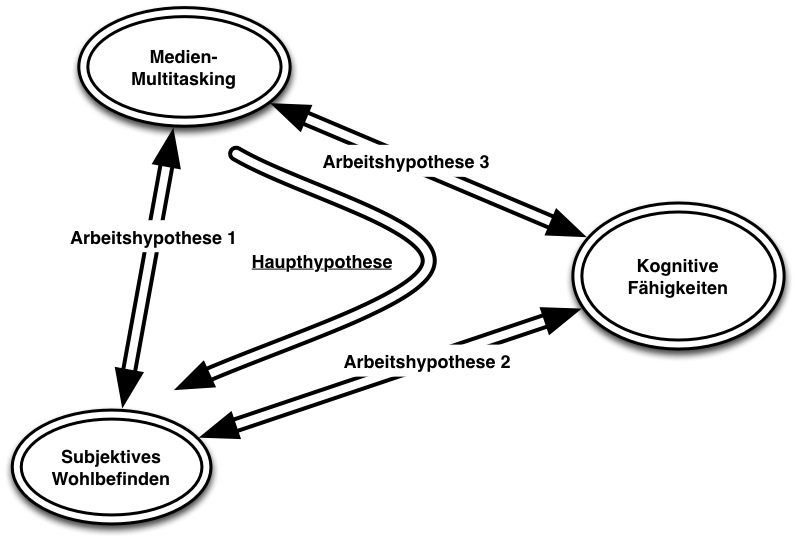
\includegraphics[scale=0.55]{images/grafiken/Hypothesen_Grafisch_v2.jpg}
     \caption{Zusammenhang Hypothesen}
     \label{pic.einleitung.hypothesen}
\end{figure}




